\subsection{Ca sử dụng tạo chuyến đi mặc định}
\noindent Ca sử dụng này mô tả cách người dùng tạo nhanh một chuyến đi mới chỉ với tên chuyến đi. Chuyến đi này mặc định sẽ ở chế độ riêng tư và người dùng có thể cập nhật chi tiết sau. Bảng~\ref{tab:uc_create_default_trip_spec} trình bày chi tiết đặc tả ca sử dụng, bao gồm luồng sự kiện chính, luồng thay thế, các điều kiện và yêu cầu liên quan. Các biểu đồ hoạt động, quan hệ (Bảng~\ref{tab:uc_create_default_trip_diagrams}) và tuần tự (Hình~\ref{fig:3-3-11-sequence-diagram}) minh họa rõ hơn về quy trình và tương tác hệ thống.
% \vspace{0.5cm} % Adjust spacing if needed

% Use longtable environment
% Need \usepackage{longtable} and \usepackage{calc} in preamble
\begin{longtable}{| p{4cm} | p{\dimexpr\linewidth-4cm-4\tabcolsep} |} % Adjust widths as needed
    \caption{Đặc tả ca sử dụng tạo chuyến đi mặc định} % Caption inside longtable
    \label{tab:uc_create_default_trip_spec} \\ % Label after caption

    \hline
    \textbf{Mô tả} & Người dùng có thể tạo chuyến đi để lên kế hoạch du lịch cho bản thân và bạn bè. \\
    \hline
    \endfirsthead % Header for the first page

    % No \endhead content needed

    % No \endfoot content needed

    \hline % Footer for the last page
    \endlastfoot

    % --- Table Content ---
    \textbf{Luồng cơ bản} & 1. Người dùng bấm vào tab chuyến đi. \newline
                           2. Người dùng bấm vào dấu ``+'' góc phải trên. \newline
                           3. Hệ thống hiển thị hộp thoại yêu cầu người dùng nhập tên cho chuyến đi. \newline
                           4. Người dùng nhập tên chuyến đi. \newline
                           5. Người dùng bấm ``Tạo". \newline
                           6. Hệ thống tạo một chuyến đi mới với tên đã đặt. \\
    \hline
    \textbf{Luồng thay thế} & Hệ thống thông báo lỗi khi tên chuyến đi dài hơn 80 kí tự. \\
    \hline
    \textbf{Tiền điều kiện} & - Người dùng đang đăng nhập và phiên đăng nhập chưa kết thúc. \\
    \hline
    \textbf{Hậu điều kiện} & - Hệ thống thêm chuyến đi với trạng thái là riêng tư của người dùng vào cơ sở dữ liệu. \\
    \hline
    \textbf{Yêu cầu phi chức năng} & Hệ thống tạo chuyến đi dưới 2s. \\
    % --- End Table Content ---

\end{longtable}


\begin{table}[H] % Wrap the diagrams table
    \centering
    \caption{Biểu đồ hoạt động và quan hệ ca sử dụng tạo chuyến đi mặc định} % Add caption
    \label{tab:uc_create_default_trip_diagrams} % Add label
    \begin{tabular}{| c | c |}
        \hline
        \textbf{Biểu đồ hoạt động} & \textbf{Quan hệ} \\
        \hline
        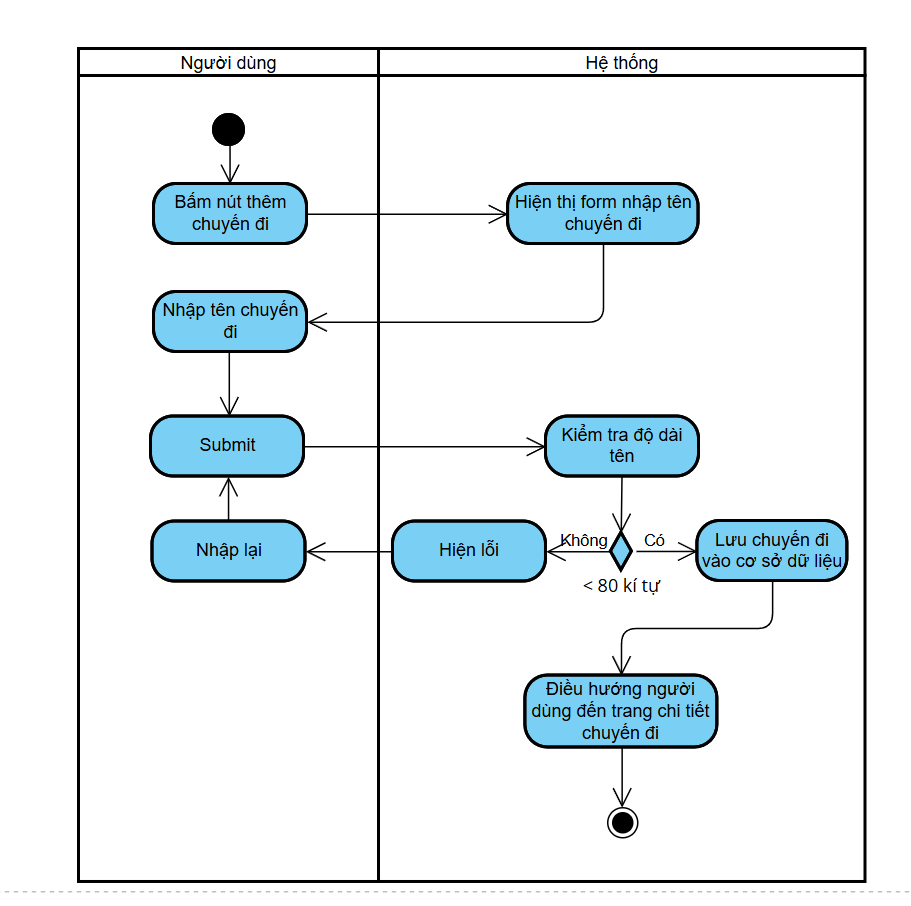
\includegraphics[width=0.5\linewidth]{figures/c3/3-3-11-ad.png} % Specified width
        &
        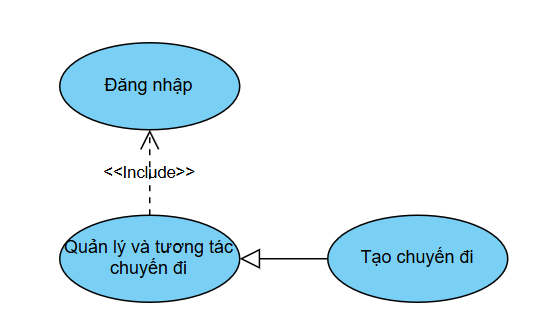
\includegraphics[width=0.45\linewidth]{figures/c3/3-3-11-rd.png} \\ % Specified width
        \hline
    \end{tabular}
\end{table}

\begin{figure}[H]
    \centering
    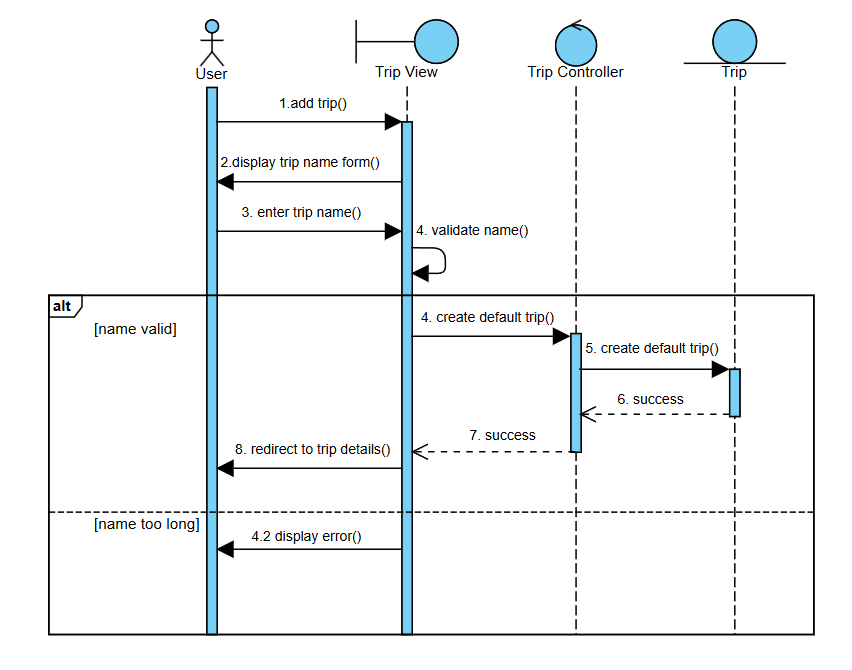
\includegraphics[width=0.95\textwidth]{figures/c3/3-3-11-sd.png} % Specified width
    \caption{Biểu đồ tuần tự ca sử dụng tạo chuyến đi mặc định.}
    \label{fig:3-3-11-sequence-diagram}
\end{figure}